\documentclass[12pt]{report}

\usepackage[italian]{babel}
\usepackage[T1]{fontenc}
\usepackage[utf8]{inputenc}
\usepackage[Algoritmo]{algorithm}
\usepackage[noend]{algpseudocode}
\usepackage[pdftex]{graphics}
\usepackage{graphicx}
\graphicspath{/home/paologio/Documenti/Università/Tesi/Malchiodi/ACSDI/Elaborato}
\usepackage{chngcntr}
\counterwithout{footnote}{chapter}
\usepackage{booktabs}
\usepackage{cite}
\usepackage{amsmath}
\usepackage{amsfonts}
\usepackage{amssymb}
\usepackage{mathrsfs}
\usepackage{amsmath}
\usepackage{amsthm}
\usepackage{bm}
\usepackage{mathtools}
\setlength
\fboxsep{0.25cm}
\usepackage[makeroom]{cancel} %\cancelto{\infty}{}
\usepackage{enumerate}
\usepackage{enumitem}
\usepackage[showframe=false]{geometry}
\usepackage{changepage}
\usepackage{pdfpages}
\usepackage{float}

\begin{document}


\includepdf{Frontespizio_UniMi.pdf}

\tableofcontents

\linespread{1.4}\selectfont

\chapter*{Introduzione}
Negli ultimi anni è aumentato l'interesse per lo studio e per l'utilizzo di algoritmi per l'apprendimento automatico (machine learning). Tali procedure hanno la perculiarità di apprendere informazioni direttamente dai dati, continuando a migliorare le prestazioni in maniera adattiva con l'aumentare degli esempi presi in considerazione. Infatti cambia l'approccio rispetto ai classici programmi: non è più il programmatore che attraverso il codice sorgente dà le istruzioni da eseguire alla macchina ma la macchina stessa che, elaborando un insieme di dati (dataset) tramite algoritmi di machine learning, sviluppa una propria logica per svolgere il compito richiesto.
L'impiego che ne viene fatto è vasto: dalla sicurezza dei dati al trading finanziario, dal campo sanitario all'elaborazione del linguaggio naturale. Con l'aumentare delle prestazioni dei processori e delle dimensioni della memoria di dispositivi mobili, questi algoritmi hanno cominciato a essere impiegati anche su dispositivi mobili e nell'IoT \footnote{Internet Of Things: termine che indica l'esistenza di una varietà di oggetti (things) che, attraverso la rete (internet) sono capaci di interagire tra di loro e collaborare con altri oggetti per creare nuovi servizi/applicazioni ~\cite{IOT}.}; oggi infatti negli smartphone ci sono programmi che, facendo uso di tecniche di machine learning, riescono ad esempio a classificare immagini o a fungere da assistente interagendo tramite comandi vocali con l'utente. 
In questo elaborato verrà preso in esame un particolare strumento usato nel machine learning, noto come reti neurali artificiali. Tale strumento sarà applicato al problema della regressione. \\
Nel primo capitolo verrà spiegato cosa sia effettivamente una rete neurale cominciando da alcuni accenni storici, fino a illustrarne l'architettura e le modalità di utilizzo. Un grande problema delle reti neurali è la quantità di memoria che viene richiesta per memorizzare le strutture dati occorrenti al loro funzionamento. A tal proposito vengono proposti due algoritmi di compressione, di cui si parlerà nel secondo capitolo, per rimediare a tale problema. L'interrogativo a cui questo elaborato si pone di rispondere è infatti quanto l'azione di compressione delle reti possa inficiare sull'accuratezza delle loro previsioni, e in merito a ciò il terzo capitolo riporta gli esiti di alcuni esperimenti di compressione effettuati su una rete che predice l'indice di inserimento di un elemento all'interno di una lista ordinata (problema del predecessore).
La parte conclusiva è dedicata all'analisi dei risultati ottenuti negli esperimenti proposti nel capitolo precedente.


\chapter{Le reti neurali artificiali}

\section{Definizione e origini storiche}
L’intuizione di replicare l’attività neurale che avviene nel sistema nervoso centrale umano quando apprende risale agli inizi degli anni ‘40, quando venne teorizzato un primo modello di neurone da McCulloch e Pitts ~\cite{McCulloch}. Il parallelo è molto stretto: così come il compito di un neurone è quello di ricevere, elaborare e ritrasmettere impulsi elettrici all’interno del sistema nervoso centrale, quello di un neurone artificiale è ricevere un certo dato in input e attivarsi o meno a seguito della sua elaborazione.
È interessante notare che, a differenza di un classico software, la costruzione di un neurone artificiale non richiede la scrittura di un programma esplicito ma avviene a seguito di un processo assimilabile a quello dell'apprendimento ~\cite{Rosenblatt}. Inoltre, continuando l'analogia con il sistema nervoso centrale, non ci si è limitati a usare un singolo neurone ma più neuroni e più strati di neuroni collegati tra loro: questo ha portato allo sviluppo delle reti neurali.


\section{Il neurone artificiale}
La Figura \ref{neuronImage} illustra il classico modello del neurone artificiale, che è composto da:
\begin{itemize}
\item{uno o più input $x_1$, $x_2$, $\dots$, $x_n$};
\item{uno o più pesi $w_1$, $w_2$, $\dots$, $w_n$};
\item{funzione d'attivazione $f$};
\item{un output}.
\end{itemize}

In particolare un neurone può essere attivato in base alla propria funzione d'attivazione: questa può essere una funzione binaria, come nel caso di quella a scalini \footnote{$\mathrm{step}(x) =
\bigg \{
\begin{array}{rl}
0 & x < 0 \\
1 & x \geq 0 \\
\end{array}
$} che attiva o disattiva il neurone, o generare un certo grado d'attivazione, come nella funzione sigmoide \footnote{$\displaystyle \mathrm{sigmoid}(x) = \frac{1}{1 + e^{-x}}$} o ReLu, che verrà spiegata nel Paragrafo \ref{relu}.

\begin{figure}[H]
\begin{center}
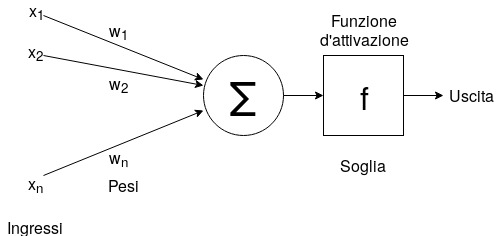
\includegraphics[scale=0.75]{neurone_artificiale.png}
\caption{Modello di un neurone artificiale}
\label{neuronImage}
\end{center}
\end{figure}

In particolare, il valore di uscita indicato nella Figura \ref{neuronImage} viene calcolato moltiplicando ogni input ($x_1$, $x_2$, $\dots$, $x_n$) per il corrispondente peso ($w_1$, $w_2$, $\dots$, $w_n$), sommandone poi i risultati; il risultato costituirà l'argomento della funzione d'attivazione ($f$). Ad esempio, considerando l'immagine seguente:
\null\par\null

\begin{figure}[H]
\begin{center}
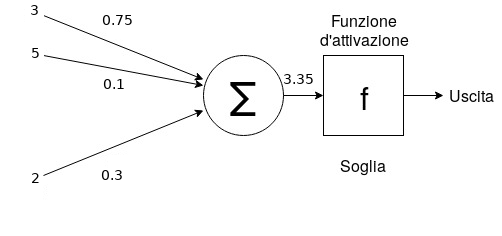
\includegraphics[scale=0.75]{neurone_artificiale_esempio_pratico.png}
\label{neuronImage}
\end{center}
\end{figure}

viene calcolato: $$3 \times 0.75 + 5 \times 0.1 + 2 \times 0.3 = 3.35$$ che verrà successivamente utilizzato come argomento nella funzione d'attivazione
$$\mathrm{Uscita} = f(\mathrm{3.35})$$
ottenendo così il valore Uscita.
\newpage
\section{Architettura di una rete neurale} \label{architettura}
Come detto precedentemente, una volta costruito un neurone artificiale, il passo successivo è stato quello di usare più neuroni in modo da formarne degli strati e connettere più strati tra di loro, in modo da permettere di affrontare problemi più complessi, compito impossibile per un neurone singolo. L'organizzazione di tale struttura può essere fatta in modi diversi, come ad esempio le reti di Hopfield ~\cite{Hopfield} o quelle convoluzionali ~\cite{Convolutional}; l'elaborato si concentrerà sull'organizzazione multistrato.
Una rete, per essere in grado di apprendere teoricamente qualsiasi funzione, deve essere composta da almeno tre strati, illustrati in Figura \ref{ReteNeuraleDensamenteConnessa}, che prendono il nome di:
\begin{enumerate}
\item{input};
\item{hidden};
\item{output}.
\end{enumerate}

\begin{figure}[H]
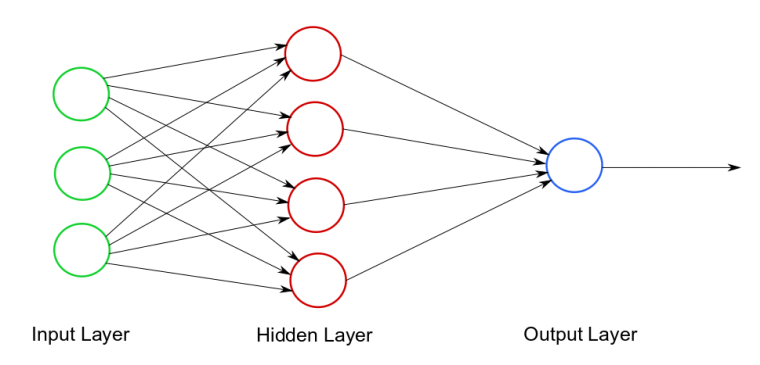
\includegraphics[scale=0.5]{nn_arch.png}
\caption{Architettura di una rete neurale multistrato}
\label{ReteNeuraleDensamenteConnessa}
\end{figure}

Il ruolo dello strato di input è quello di ricevere le feature da elaborare, lo strato nascosto si occuperà di costruire una rappresentazione intermedia delle feature, che verrà poi elaborata dallo strato di output per fornire il risultato.

Inoltre, in base a come i neuroni dei vari strati sono collegati tra loro, si possono distinguere diverse configurazioni di rete come quella densamente connessa (fully connected), convoluzionale (convolutional) \footnote{a differenza di quelle densamente connesse, i neuroni di uno strato sono collegati solo a una piccola parte dello strato precedente ~\cite{Convolutional}.} usata principalmente per il riconoscimento di pattern in immagini o ancora quella ricorrente \footnote{la particolarità è che l'architettura prevede che siano presenti delle connessioni tra neuroni di uno strato e quello precedente, perdendo così la caratteristica di grafo aciclico; è usata quando è importante l'ordine dei dati, ad esempio nel riconoscimento del parlato o per riconoscere sequenze di stringhe o frame di un video ~\cite{Recurrent}.} .
In questo elaborato ci si concentrerà sulla tipologia densamente connessa, in cui ogni neurone di uno strato sarà collegato a ogni neurone di quello successivo, come mostrato in Figura \ref{ReteNeuraleDensamenteConnessa}.

Come detto sopra, la rete è composta da strati; gli strati, a loro volta, sono un insieme di neuroni, ognuno dei quali ha associato un peso ($w$) per ogni collegamento in entrata e un bias ($b$). Questi devono essere prima inizializzati ~\cite{ParametersInitialization}; esistono diversi modi di farlo (ad esempio estraendo valori da una distribuzione uniforme o gaussiana): negli esperimenti condotti sono stati inizializzati casualmente, seguendo una distribuzione uniforme in $[0, 1)$. Questi due sono gli unici parametri che, una volta inizializzati, vengono modificati automaticamente dalla rete durante il training. I restanti parametri, come il numero di neuroni in uno strato hidden o il numero di strati, rimangono tali durante tutte le fasi di addestramento del modello; inoltre l'approccio tipicamente usato per individuare tali parametri, che prendono il nome di \textit{iperparametri}, è quello empirico, e di esso si parlerà nel Paragrafo \ref{iperparametri}.

\section{Applicazioni}
Le reti neurali vengono impiegate principalmente nell’attività di previsione (regressione) o classificazione.
Nel primo caso rientrano, ad esempio, le previsioni di vendita: riuscire a prevedere il prezzo di un immobile in base a fattori che lo descrivono (i metri quadrati, il numero di stanze, la posizione centrale o meno in un centro abitato, ecc…) o prevedere l’andamento di un titolo azionario in borsa.
Altro problema è quello invece della classificazione: si richiede in questo caso che la rete, dato un oggetto, ne restituisca la classe di appartenenza; tipico esempio è quello della classificazione di numeri scritti a mano o, date una serie di immagini, riconoscere quelle in cui è presente un particolare soggetto.
In questo elaborato si andrà ad affrontare il problema legato alla regressione.

\section{Esecuzione di una rete feed-forward}
Le connessioni tra i neuroni di uno strato e quelli del successivo sono monodirezionali, configurazione che porta ad avere un grafo diretto e aciclico. Quindi il flusso di dati che scorre nella rete viaggia dallo strato di input a quello di output senza che ci siano cicli, il che implica anche che non ci siano interazioni tra neuroni dello stesso strato e che il tempo necessario per far scorrere i dati da input a output sia costante, dato che i vari neuroni elaborano parallelamente i segnali che ricevono.

\subsection{Il calcolo tra strati}\label{feedforward}
Nell'implementazione pratica i pesi delle connessioni vengono rappresentati da matrici  e i pesi dei bias da vettori. 
Siano:
\begin{itemize}
\item{$W_{ih}$} la matrice dei pesi di dimensione $r \times c$, dove $r$ è il numero di neuroni in input e $c$ il numero di neuroni dello strato hidden; ogni componente di questa matrice rappresenta il peso di una connessione tra un neurone dello strato input e uno dello strato hidden;
\item{$W_{ho}$} analogamente al punto precedente, la matrice dei pesi che rappresenta le connessioni tra gli strati nascosto e di output;
\item{$b_h$} il vettore colonna dei bias dello strato hidden di dimensione $r \times 1$ dove $r$ è il numero di neuroni dello strato hidden; ogni componente rappresenta il bias di uno dei neuroni dello strato hidden;
\item{$b_o$} analogamente al punto precedente, il vettore dei bias dello strato di output;
\item{$x$} il vettore di input;
\item{$f$} la funzione d'attivazione scelta per lo strato.
\end{itemize}
Per eseguire l'algoritmo di feed-forward occorre calcolare
$$\alpha = f\left(x \cdot W_{ih} + b_h\right),$$
procedendo poi analogamente con lo strato successivo
$$\mathrm{prediction} = f\left(\alpha \cdot W_{ho} + b_o\right).$$
Da notare che, in entrambi i casi sopra, la funzione d'attivazione viene applicata a ogni componente del vettore. Inoltre, per semplicità, nell'esempio è stata usata la stessa $f$ per ogni strato; nulla vieta però di applicare una funzione di attivazione diversa per ogni strato.
Le reti considerate in questo lavoro vengono utilizzate per calcolare una regressione, e dunque hanno un solo neurone di output: prediction sarà quindi un valore scalare che rappresenterà la previsione della rete in base all'input ricevuto.
\newpage
\section{Addestramento di una rete neurale}
Per continuare il parallelo con il sistema nervoso centrale umano, così come per l'attività di apprendimento occorre studiare, anche una rete neurale artificiale ha bisogno di ``studiare'': questa fase viene detta fase di addestramento (training).
Una volta selezionato il dataset contenente un certo numero di esempi \footnote{un esempio è rappresentato da un insieme di feature e un target.}, si procede a dividere tale insieme in due sottoinsiemi: per fare questo, negli esperimenti che verranno presentati più avanti, si è utilizzato un holdout di 80\% - 20\% rispettivamente per training set, che verrà usato per l'attività di apprendimento, e per il testing set, per valutare la bontà della rete su esempi che non ha ancora visto.
Una soluzione alternativa sarebbe stata quella di fare una cross-validation, concetto spiegato nel Paragrafo \ref{crossvalidation}.

\subsection{Fase di training}
In questa fase le feature degli esempi nel training set vengono copiate nello strato di input della rete. Utilizzando la procedura descritta nel Paragrafo \ref{feedforward}, la rete propaga il risultato fino al neurone di output. È in questo momento che la rete impara confrontando la previsione con l’effettivo target: in base alla loro differenza, la rete stessa correggerà i pesi degli strati usando un algoritmo noto come back-propagation (spiegato nel Paragrafo \ref{backprop}), con l'obiettivo di minimizzare localmente una funzione di perdita \label{loss} (loss function) \footnote{in questo caso è la funzione legata all'errore di predizione fatto dalla rete sui dati del training set.}.
L'operazione di aggiornamento dei pesi viene in realtà eseguita solo dopo che un certo numero di esempi è stato mostrato alla rete: tale numero prende il nome di batch size. Normalmente è necessario effettuare vari cicli di aggiornamento che richiedono di mostrare gli esempi del training set più volte, questo concetto prende il nome di epoca, che indica quante volte la rete ha visto ogni esempio.
Se per esempio si avessero 200 esempi nel training set e un batch size pari a 10, ciò significherebbe che l'aggiornamento dei pesi avverrebbe ogni volta che sono stati presentati alla rete 10 esempi, e
quindi un'epoca corrisponderebbe a $200 \div 10 = 20$ aggiornamenti. Ipotizzando che l'intero processo di addestramento richieda cento epoche, si ottiene quindi che l'aggiornamento dei pesi è stato effettuato $20 \times 100 = 2000$ volte.

Inoltre esistono diversi criteri per stabilire quando terminare l'apprendimento; in particolare negli esperimenti condotti in questo elaborato ne sono stati usati due basati su:
\begin{itemize}
\item{epoche}: il processo di apprendimento prosegue fino al raggiungimento del numero di epoche predefinito;
\item{valore della loss function}: vengono fissate due soglie, $s_1$ e $s_2$; l'apprendimento termina quando la loss function non supera $s_1$ per $s_2$ volte consecutive.
\end{itemize}

\subsection{Fase di testing}
Terminata la fase di training occorre verificare il comportamento della rete su dati nuovi rispetto a quelli usati per addestrarla. Questo permette di valutare la reale capacità di previsione della rete e di valutare se durante l'addestramento si sia verificato uno dei problemi descritti di seguito.
\begin{itemize}
\item{si parla di \textit{overfitting} quando il modello si adatta così tanto agli esempi del training set da perdere la capacità di generalizzare su nuovi esempi. Sintomo dell'overfitting è un'alta accuratezza durante la fase di training e una scarsa accuratezza in fase di testing; la rete ha imparato ``a memoria'' i casi di training in modo tale da non riconoscerne di nuovi};
\item{l'\textit{underfitting} è l'opposto del caso precedente. Si verifica quando il modello non riesce a imparare la relazione tra feature e target, risultando in previsioni poco accurate}.
\end{itemize}

\section{Algoritmo di back-propagation}\label{backprop}
L'apprendimento consiste nel determinare i pesi delle connessioni e i bias che permettono alla rete di fare predizioni accurate sul training set. In altre parole bisogna minimizzare l'errore quadratico medio di predizione, che è la loss function citata nel Paragrafo \ref{loss}.
Il numero di argomenti della funzione da ottimizzare è molto elevato, e inoltre questa funzione è non-lineare, quindi non si possono utilizzare le tecniche classiche di ottimizzazione. La soluzione a questo problema consiste nell'utilizzare una tecnica locale e iterativa, nota come back-propagation ~\cite{Backpropagation}, che regola i pesi e i bias associati ai collegamenti. Quello che permette di fare è legare l'errore ottenuto in output da una rete neurale a un algoritmo di ottimizzazione locale di una funzione di errore, in questo caso l'errore quadratico medio di predizione degli esempi del training set. L'algoritmo utilizzato è quello del gradiente discendente che consiste nel modificare i parametri della rete sottraendo loro una frazione del gradiente \footnote{data una funzione $f$ e i suoi parametri $x$ e $y$, il gradiente della funzione $f(x, y)$, indicato con $\nabla f(x, y)$, è dato dal vettore $[\frac{\partial f}{\partial x}, \frac{\partial f}{\partial y}]$.}.
Per l'aggiornamento del peso viene usata la seguente formula:
$$W^n_x = W_x - \eta \left(\frac{\partial \mathrm{Error}}{\partial W_x}\right)$$ dove $W^n_x$ è il nuovo valore del peso, $W_x$ il vecchio peso, $\eta$ il learning rate \footnote{valore solitamente vicino allo 0; è il grado con cui la rete adatta i propri pesi, più è alto il learning rate e più impatto avrà l'errore propagato e viceversa.} e $\frac{\partial \mathrm{Error}}{\partial W_x}$ la derivata parziale dell'errore rispetto ai pesi. 

Una volta fatto questo calcolo con la matrice dei pesi strato hidden/output, si fa la stessa cosa per quella input/hidden. Il procedimento descritto viene iterato per tutta la durata dell'allenamento della rete al termine della fase della visione di un intero batch.

Un problema legato a questo algoritmo è che è possibile rimanere bloccati in un punto di minimo locale, dato che l'algoritmo di ottimizzazione usato è locale. Questo succede quando la funzione presenta un punto di minimo locale in un intorno sufficientemente grande da impedire ai passi compiuti nella discesa del gradiente di spostarsi da quel punto. Non sempre però è un grave problema, può accadere ad esempio che il valore che minimizza un punto di minimo locale si comporta bene quasi come quello che minimizza il minimo globale, come in Figura \ref{localMinima}. Per evitare di rimanere bloccati su un minimo locale si possono provare diverse soluzioni come aumentare il valore del learning rate, incrementare il numero di strati nascosti o ancora provare diverse funzioni d'attivazione o algoritmi di ottimizzazione diversi dalla discesa del gradiente ~\cite{LocalMinima}.

\begin{figure}[H]
\begin{center}
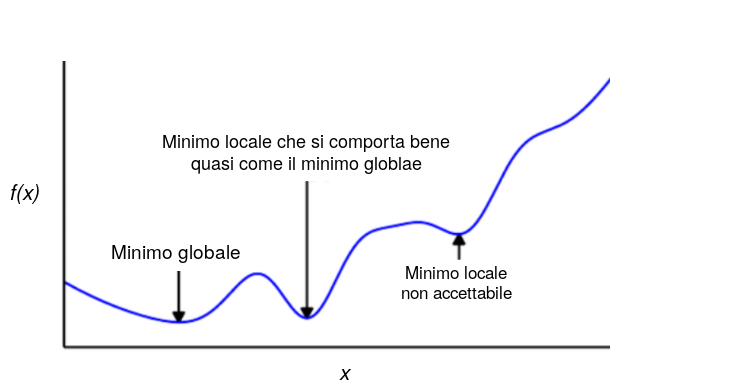
\includegraphics[scale=0.5]{localMinima.png}
\caption{Diversi punti di minimo in una funzione}
\label{localMinima}
\end{center}
\end{figure}

\subsection{Iperparametri}\label{iperparametri}
Gli iperparametri, di cui si è già accennato nel Paragrafo \ref{architettura}, sono caratterizzati dal fatto che il loro valore viene impostato prima che l'addestramento abbia inizio e che non cambiano nel corso dello stesso. Negli esperimenti presentati in questo elaborato questi valori vengono selezionati empiricamente attraverso model selection (vedi Paragrafo \ref{modelselection}).
In questa categoria rientrano:
\begin{itemize}
\item{learning rate}: indica il grado con cui la rete modifica i propri pesi durante la fase di back-propagation;
\item{numero di epoche}: indica il numero di volte che la rete ha visto tutti gli esempi del training set;
\item{batch size}: indica dopo quanti esempi mostrati alla rete si aggiornano i pesi;
\item{numero di neuroni per strato nascosto \footnote{in questo elaborato verranno usate reti neurali con zero, uno e due strati nascosti: per casi più complessi si può arrivare ad un numero maggiore di strati nascosti.}}: indica il numero di neuroni per singolo strato;
\item{funzione d'attivazione}: funzione che determina l'intensità d'attivazione del singolo neurone.
\end{itemize}

Ogni volta che in questo elaborato verranno introdotti nuovi esperimenti ne verranno anche indicati gli iperparametri relativi.

\section{Model selection}\label{modelselection}
Come indicato nel Paragrafo \ref{iperparametri}, per trovare il valore degli iperparametri bisogna basarsi su prove empiriche. In particolare, negli esperimenti condotti sono stati fissati a priori i valori per numero di epoche, batch size, numero di strati nascosti, learning rate e funzione d'attivazione. Il numero di neuroni dello strato nascosto è stato dimensionato usando una tecnica di model selection che prende il nome di cross-validation che verrà spiegata nel prossimo paragrafo.

\subsection{Cross validation}\label{crossvalidation}
Dopo aver diviso il training set dal testing set, viene utilizzato esclusivamente  il primo per la cross-validation. In particolare questo viene partizionato in $k$ sottoinsiemi (fold \footnote{l'idea è quella di suddividere gli $m$ esempi in $k$ gruppi di grandezza approssimativamente uguale, per semplicità si è deciso di mettere i primi $\frac{m}{k}$ elementi del training set nel primo fold e così via.}) di cui uno di questi prenderà il nome di validation set e gli altri di training set. Per ogni valore possibile dell'iperparametro (o per ogni possibile configurazione se ci sono più iperparametri) vengono ripetuti $k$ processi di addestramento, ogni volta eliminando dal training set uno dei fold e utilizzando quet'ultimo per calcolare l'errore; si ottengono così $k$ errori di cui si calcola la media.

Se per esempio il training set venisse suddviso in tre fold, le permutazioni prese in considerazione saranno quelle descritte nella Figura \ref{foldDiagram}.

\begin{figure}[H]
\begin{center}
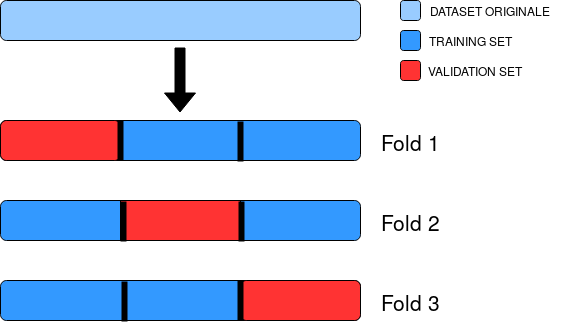
\includegraphics[scale=0.45]{foldDiagram.png}
\caption{Divisione di un dataset in 3 fold}
\label{foldDiagram}
\end{center}
\end{figure}

Viene infine scelto il valore dell'iperparametro (o degli iperparametri) che corrisponde all'errore medio minore, per poi riaddestrare la rete e valutare la bontà di generalizzazione di quest'ultima utilizzando il test set.

Di seguito è presentato l'algoritmo di cross validation in pseudocodice; per semplicità se ne presenta una versione in cui si fa cross validation su un solo iperparametro, ma lo stesso algoritmo può essere usato per più iperparametri.

\makeatletter
\def\BState{\State\hskip-\ALG@thistlm}
\makeatother
\begin{algorithm}
\caption{Cross Validation}
\begin{algorithmic}[1]
\BState \emph{input}:
\State $H \gets \textit{insieme dei valori di un iperparametro}$
\State $S \gets \textit{training set}$
\State $K \gets \textit{numero di fold}$
\BState \emph{procedura}:
\State $L[h] \gets 0 \;\forall\; h \;\in\; H$\\

\For {$h \in H$}

\For {$k \in \{1,\dots,K\}$}
\State $s_{k} \gets \textit{k-esimo fold di S}$

\State $\textit{alleno la rete su } S \setminus s_{k}$
\State $\textit{valuto la rete su } s_{k}$
\State $L[h] \gets L[h] + \textit{valore di loss per il k-esimo fold per h-esimo iperparametro}$
\EndFor
\State $L[h] \gets L[h] \div K$
\EndFor
\State $h_{best} \gets arg_min(L[h]\, \forall\, h \in H )$
\State $\textit{return}\, h_{best}$
\end{algorithmic}
\end{algorithm}

\chapter{Algoritmi di compressione per reti neurali}

\section{Compressione di una rete}

Uno degli svantaggi più evidenti delle reti neurali è lo spazio che queste occupano in memoria e i tempi elevati per il loro addestramento. Questo aspetto ha assunto un ruolo sempre più importante con il diffondersi di macchine con ridotte capacità di computazione e di memoria e in generale dell’IoT. 
Per ridurre questo impatto negativo si stanno studiando diverse soluzioni tra cui comprimere le strutture dati alla base di una rete neurale in modo da ridurne le dimensioni in memoria intaccandone il meno possibile l'accuratezza. Questo elaborato si prefigge di verificare l'efficacia di due tecniche di compressione note come ``pruning'' e ``weight sharing'' su una rete neurale feed-forward utilizzata per problemi di regressione.

\section{Pruning}\label{pruning}

L’idea di fondo del pruning è semplice: ogni collegamento tra neuroni ha associato un peso che ne determina l’importanza (avrà letteralmente un peso maggiore nell’influenzare il risultato finale della rete quando il valore della connessione è molto alto o molto basso); da qui l’intuizione per cui, ignorando i collegamenti con peso tendente allo zero, non si altera significativamente il risultato della rete che si otterrebbe considerandoli ~\cite{Pruning}.
Questo risultato si può ottenere azzerando tali connessioni, ossia mettendo a zero il valore nella matrice dei pesi relativo alla connessione che si intende eliminare. Facendo così però si ottiene solo una parte del risultato che si vuole raggiungere usando il pruning; essendo il valore a zero si potrà verificare l'accuratezza della rete prunata di una percentuale di connessioni, ma non si godrà della riduzione di memoria, in quanto la matrice avrà lo stesso numero di elementi e quindi bisogno dello stesso numero di byte in memoria. Per questo viene in aiuto una particolare struttura dati adatta alla rappresentazione di matrici sparse \footnote{per matrice sparsa si intende una matrice con un numero consistente di valori nulli.}. 
Due scelte possibili per la struttura dati che accoglie la matrice sparsa sono indicate di seguito.
\begin{itemize}
\item{\textbf{\textit{compressed sparse row}}} ~\cite{CSC}: vengono usati 3 vettori contenenti rispettivamente i valori non nulli della matrice letti riga per riga, gli indici di colonna e i puntatori ai primi valori non nulli delle righe descritti nel modo seguente: 

$$ptr =
\bigg \{
\begin{array}{ll}
ptr[0] = 0 \\
ptr[i] = prt[i - 1] - nz \\
\end{array}
$$
dove $nz$ è il numero di elementi non nulli nella riga $i - 1$;

\item{\textbf{\textit{compressed sparse column}}}: simile alla precedente con la differenza che nel primo vettore i valori vengono letti per colonna, vengono memorizzati gli indici di riga per ogni valore e i relativi puntatori alle colonne.
\end{itemize}

Tuttavia questa operazione non è del tutto gratuita: l'operazione di moltiplicazione tra matrice e vettore con queste nuove strutture dati compresse è più lenta.
Ne viene proposta l'implementazione in pseudocodice:

\null\par\null

\makeatletter
\def\BState{\State\hskip-\ALG@thistlm}
\makeatother
\begin{algorithm}
\caption{Moltiplicazione CSC per vettore}
\begin{algorithmic}[1]
\BState \emph{Siano}:
\State $val \gets \textit{vettore contenente i valori non nulli}$
\State $col \gets \textit{vettore contenente gli indici di colonna}$
\State $row\_ptr \gets \textit{vettore contenente i puntatori alle righe}$
\State $x \gets \textit{vettore da moltiplicare}$
\State $N \gets \textit{numero di colonne del vettore x}$
\State $y \gets \textit{vettore risultate}$
\For {$i \in N$}
\For {$j \in \{row\_ptr[i],\dots,row\_ptr[i + 1]\}$}
\State $y[i] \gets y[i] + val[j] \times x[col[j]]$
\EndFor
\EndFor
\end{algorithmic}
\end{algorithm}

\newpage

\subsection{Tasso di compressione}

Il tasso di compressione ottenuto mediante pruning si può calcolare notando che quello che cambia è il numero di connessioni che vengono mantenute rispetto a quelle della rete originale. Denotando quindi con $\tau$ la soglia utilizzata \footnote{In questo elaborato la soglia per scartare i pesi è stata calcolata come $n$-esimo percentile rispetto alla distribuzione dei pesi nella matrice, per $n \in \{10, \dots, 90 \}$ (quindi per $n=10$ verranno scartate il 10\% circa delle connessioni tra due strati comunicanti e così via).}, $s_c$ lo spazio occupato dalla rete compressa composta dai pesi $\lbrace w_{ij} \,|\, w_{ij} \geq \tau \rbrace$ e $s$ lo spazio occupato dalla rete originale, la percentuale di memoria risparmiata può essere espressa tramite l'equazione

\begin{equation}
\mathrm{ratio} = \frac{s_c}{s}
\end{equation}

Tuttavia, come si vedrà alla fine del Paragrafo \ref{CSRProblem}, questo è un risultato teorico che non tiene conto del variare della struttura dati utilizzata. Occorre infatti notare che al di sotto di una certa percentuale di pruning l'uso di una struttura dati, quale la CSR, non è conveniente in termini di memoria occupata.

\newpage

\section{Weight Sharing}

La tecnica del weight sharing prende spunto dal flyweight pattern ~\cite{GOF}: questo è uno strumento di ingengeria del software che permette di ottimizzare la memoria utilizzata facendo condividere un oggetto usato da più istanze piuttosto che crearne più copie. Un esempio concreto potrebbe essere quello riportato nel testo citato sopra, ossia quello di un editor di testo. Occorre distinguere però i due stati dell'oggetto condiviso, quello \textit{interno}, che fa riferimento alle qualità intrinseche dell'oggetto indipendenti dall'utilizzo che ne verrà fatto, e quello \textit{esterno}, che fa riferimento a quelle caratteristiche dipendenti dal contesto che possono mutare senza che muti l'oggetto condiviso. Tornando all'esempio dell'editor di testo, lo stato interno dell'oggetto condiviso è il carattere, mentre quello esterno la posizione all'interno del testo. Una volta creato un oggetto che raggruppi tutte le lettere dell'alfabeto, occorre interrogare tale oggetto condiviso per avere un riferimento alla lettera da inserire nel testo, operazione che chiede meno spazio rispetto alla creazione di un nuovo oggetto carattere ogni volta. 

Nel caso pratico di una rete neurale l'oggetto condiviso è un array e le lettere dell'alfabeto sono i \textit{centroidi}. Il centroide è un valore che rappresenta alcuni valori simili delle matrici dei pesi che vengono raggruppati in questo singolo valore. Questo valore viene usato in sostituzione ai pesi raggruppati per le operazioni matriciali. Come per l'esempio dell'editor di testo anche qui si possono distinguere uno stato interno, il valore numerico del centroide, e uno stato esterno, la posizione all'interno della matrice, o in altre parole il peso della connessione.
Per stabilire i centroidi si possono usare algoritmi di clustering; in particolare quello usato in questo elaborato è K-Means ~\cite{KMeans}, che verrà spiegato nel dettaglio nel Paragrafo \ref{kmeans}. \\

\subsection{Tasso di compressione}
Come strutture dati sono stati utilizzati un vettore per ogni strato in cui vengono memorizzati i centroidi usando valori float a 32 bit e una matrice in cui memorizzare l'indice del centroide relativo; gli indici sono rappresentati da interi a 16 bit se la dimensione della matrice è superiore a 256, altrimenti da interi a 8 bit. \\
Il tasso di compressione, $\eta$, ottenuto tramite la tecnica del weight sharing è espresso dalla seguente formula:
\null\par\null
$$
\displaystyle{\eta=\frac{n m \times f(n,m) + 32k}{32 \times n m}}
$$

$$\mathrm{dove}\,\,\,\,\,
\begin{array}{ll}
k = \mathrm{numero\, di\, centroidi}, \\
n, m = \mathrm{dimensione\, delle\, matrici}
\end{array},
f(k) =
\bigg \{
\begin{array}{rl}
16 & nm > 256 \\
8 & \mathrm{altrimenti} \\
\end{array}
$$

\null\par\null

Pertanto, il tasso di compressione per gli esperimenti trattati nell'elaborato, dopo aver fissato il numero di cluster \footnote{per cluster si intende uno degli insiemi di pesi che sono stati raggruppati: il centroide che li rappresenterà si ottiene calcolandone il valor medio.} per strato e dopo averne trovato i centroidi, le matrici dei pesi sono state sostituite con le matrici di indici che puntano al relativo centroide.

\newpage

\subsection{Algoritmo K-Means}\label{kmeans}
K-Means è un algoritmo di clustering iterativo. Si supponga di avere dei punti rappresentati su un piano cartesiano; l'obiettivo dell'algoritmo è quello di trovare dei sottogruppi di punti omogenei rispetto a una particolare misura, in questo caso la distanza euclidea ~\cite{KMeansArticle}. Esistono diverse implementazioni di questo algoritmo, tra cui l'euristica di Hartigan ~\cite{Hartigan}, quella di Lloyd ~\cite{Lloyd}; quella usata in questo elaborato è quella di Lloyd che in particolare prevede i seguenti passi:

\begin{enumerate}
\item{vengono scelti $k$ centroidi casualmente, dove $k$ è il numero di cluster che si vogliono creare};
\item{ogni osservazione viene assegnata al centroide in base alla minor distanza euclidea};
\item{i centroidi vengono aggiornati in base alla media dei valori rientranti nel cluster};
\item{se i centroidi sono stati aggiornati si ripete iterativamente dal punto 2, altrimenti l’algoritmo ha trovato i $k$ centroidi}.
\end{enumerate}

L’algoritmo usato è quello della libreria sklearn, MiniBatchKMeans ~\cite{KMeansMiniBatch} \footnote{https://scikit-learn.org/stable/modules/generated/sklearn.cluster.MiniBatchKMeans.html.}, una versione ottimizzata della precedente euristica di Lloyd che permette di lavorare, ad ogni iterazione, su un sottoinsimene preso casualmente dei dati totali.


\chapter{Esperimenti}

\section{Dataset utilizzati}
In questo paragrafo vengono descritti i dataset per i due problemi affrontati nella tesi: predizione del valore dei calciatori Fifa 2019, trattato nel Paragrafo seguente, e la predizione del predecessore in una sequenza ordinata, trattato nel Paragrafo \ref{probPred}.
Si è deciso di cominciare usando un dataset con informazioni relative alle caratteristiche dei giocatori di calcio Fifa 2019 \footnote{https://www.kaggle.com/karangadiya/fifa19, ultimo controllo 01/03/2020.}, con il problema di predire il valore di mercato del giocatore. Per tale problema è stata usata una rete neurale che sfrutta le API di Keras \footnote{https://keras.io/models/model/.}.

Una volta conclusa questa parte si è affrontato il problema della compressione per il problema del predecessore usando un dataset descritto nel dettaglio nel Paragrafo \ref{probPred}. Per quest'ultimo problema, invece, è stata creata una rete ad hoc al fine di poter sfruttare le nuove strutture dati introdotte per eseguire pruning, ovvero le matrici sparse, e weight sharing, con un vettore e una matrice per ogni strato.

D'ora in poi si utlizzerà il termine \textit{feature} per indicare una caratteristica che la rete usa durante la fase di training per predire il risultato e \textit{target} per indicare il valore da predire in base alle feature in input.

\subsection{Fifa 2019}

Il primo dataset utilizzato è quello dei giocatori Fifa, composto da 89 feature e circa 18.2k esempi; il target da predire sarà il loro valore di mercato.
Una volta eliminate le feature non necessarie all’esperimento (nome del giocatore, immagine del club, numero di maglia, ecc… ) si è proceduto a convertire tutte le feature rappresentate come stringhe (come ``Value'', ``Release clause'', ``Height'', ecc…) in float e a rimuovere dal dataset tutti gli esempi il cui ``Value'' risultasse superiore o uguale al valore minimo tra gli outlier trovati \footnote{tali outlier sono stati trovati selezionando tutti i valori standardizzati maggiori di una soglia impostata a 2.}, questo per evitare una prestazione peggiore in fase di training e testing ~\cite{Outlier}. Inoltre i nomi delle squadre di appartenenza sono stati inclusi come feature significative e codificati in valori interi.

Terminata questa fase preliminare si è deciso di considerare diverse alternative: la prima in cui vengono considerate tutte le feature a disposizione, la seconda in cui vengono selezionate solamente quelle il cui indice di correlazione \footnote{Calcolato tramite il metodo corr di pandas che utilizza il coefficiente di correlazione di Pearson $\rho_{X,Y} = \frac{cov(X, Y)}{\sigma_X\sigma_Y}$ dove $cov$ è la covarianza, $\sigma_X$ la deviazione standard di X e $\sigma_Y$ la deviazione standard di Y.} calcolato rispetto al target fosse maggiore di 0.55.
È stata considerata anche una terza opzione: selezionare la metà delle feature tramite la Principal Component Analysis (PCA) che permette di ridurre la dimensione di un insieme di dati costituito da un elevato numero di variabili interconnesse, mantenendo il più possibile la variabilità presente in esso ~\cite{PCA}. 

\subsection{Problema del predecessore in sequenze ordinate}\label{probPred}
Se si vuole mantenere una lista di elementi ordinati per poi riuscire ad accedervi in poco tempo esistono delle strutture dati dedicate come ad esempio gli alberi binari bilanciati, tra cui i B-tree e i B+-tree ~\cite{BTree}. Il tempo di accesso a queste strutture dati è dell'ordine di $O(log\,n)$, dove $n$ è il numero totale di elementi. Nonostante questo sia uno dei risultati migliori usando le strutture dati attualmente a disposizione, si è pensato di sfruttare le reti neurali per predire la posizione di un elemento all'interno di una sequenza ordinata di elementi con l'obiettivo di predire una posizione nella sequenza, data una chiave da cercare, più velocemente ma ammettendo anche un margine d'errore. \\
Formalmente, siano $x_1 \leq x_2 \leq \dots x_n$ gli $n$ elementi di input, con $x_i \in \mathbb{N}$.\\
Il problema considerato è quindi il seguente: dato $x \in X = \{x_1, x_2, \dots, x_m\}$, restituire $\mathrm{pred}(x) \in \{1, 2, \dots m\}$, posizione del predecessore di $x$ nella sequenza.
Il problema può essere risolto mediante una stima $\hat{F}$ della funzione di ripartizione empirica $F$ rispetto a $X$. La stima di $F$ viene ottenuta addestrando una rete sugli esempi $\{x_i, F(x_i)\}$, $i \in \{1, 2, \dots, m \}$; l'indice del predecessore di $x \in X$ può essere stimato mediante la formula seguente:
\begin{equation}
\mathrm{pred(x)} = \lceil\hat{F}(x)\times m\rceil
\label{empirical}
\end{equation}
Per questo problema sono stati utilizzati tre dataset, rispettivamente con $512$, $8192$ e $1048576$ esempi. Gli elementi $x_i$ sono stati rappresentati in codifica binaria. In questa versione si considereranno solamente valori di $x$ già presenti nella lista e il problema non si occuperà di operazioni di aggiornamento della lista quali inserimento ed eliminazione.

\section{Architettura delle reti}\label{architettura}
\subsection{Rete Keras per analizzare il dataset di Fifa19}
La prima rete considerata è stata costruita sfruttando delle API di Keras \footnote{https://keras.io/models/model/}. La rete è composta da uno strato di input con un numero di neuroni pari al numero di feature considerate, pari a $\lceil\log_2 m\rceil$, uno strato hidden con $n$ neuroni e uno strato di output con un singolo neurone. Per gli iper-parametri si è deciso di fissare learning rate, numero di epoche, batch size e funzione d'attivazione; per trovare il numero di neuroni per il singolo strato hidden, invece, si è usata una tecnica di model selection, modalità descritta al Paragrafo \ref{crossvalidation}.

\subsection{Rete per il problema del predecessore}\label{reteAdHoc}
Per il secondo problema sono state usate tre reti differenti:
\begin{itemize}
\item{rete 1 con 0 strati hidden};
\item{rete 2 con 1 strato hidden di 256 neuroni};
\item{rete 3 con 2 strati hidden di 256 neuroni ciascuno}.
\end{itemize}

Per tutte e tre le versioni gli iperparametri usati sono:
\begin{itemize}
\item{momentum update}\footnote{valore che è compreso tra 0 e 1 che accelera la discesa del gradiente verso il minimo globale ~\cite{Momentum}.}: $0.9$;
\item{$\lambda$}\footnote{usato per nella regolarizzazione l2, valore aggiunto alla loss function che forza pesi a scalare, penalizzando i pesi più grandi, riducendo così il problema di overfitting ~\cite{L2}.}: $10^{-5}$;
\item{batch size}: $64$;
\item{epoche}: $20000$;
\item{stop function}: vengono fissate due soglie, $s_1$ e $s_2$; l'apprendimento termina quando il valore della loss function non è inferiore a $s_1$ per $s_2$ volte consecutive; $s_1$ viene fissato inizialmente a 100 e poi aggiornato con il valore di loss più basso ottenuto e $s_2 = 4$.
\end{itemize}
Per la rete 1 è stato usato un learning rate di $5 \times 10^{-4}$, mentre per le altre due di $3 \times 10^{-3}$; questi valori sono stati trovati eseguendo un tuning sull'iperparametro notando che, per la rete senza strati nascosti, un valore più basso di learning ratge dava risultati con errore medio minore. I valori tra cui si è effettuato il tuning sono $\{5 \times 10^{-4}, 5 \times 10^{-3}, 3 \times 10^{-3}, 1 \times 10^{-3}, 1 \times 10^{-2}, 1 \times 10^{-1}\}$.

D'ora in poi ci si riferirà a queste reti come \textbf{NNX}, dove X indica il numero di strati.

\subsection{Oragnizzazione dei dati}
Per quanto riguarda il dataset Fifa, una volta mescolati gli esempi in maniera casuale, sono stati estratti l'80\% degli esempi come train set e il restante 20\% come test set. Ogni valore null all’interno dei set è stato poi sostituito con la media della relativa colonna e i valori scalati usando StandardScaler della libreria Python sklearn \footnote{https://scikit-learn.org/stable/modules/generated/sklearn.preprocessing.StandardScaler.html.} che utilizza la seguente formula:
\begin{equation}
z = \frac{x - u}{std}
\label{standardscaler}
\end{equation}
dove $u$ è la media del campione e $std$ è la sua deviazione standard.

Per il secondo dataset vengono usati tutti gli esempi nel training, dopo essere stati permutati casualmente; i target invece vengono ricavati tramite la funzione numpy linspace di Python che, dati due estremi di un intervallo e un intero $x$, restituisce un array di $x$ valori ordinati equamente spaziati compresi tra gli estremi indicati.

\subsection{Addrestramento}\label{relu}
Per scegliere il giusto numero di neuroni per lo strato hidden della rete Keras al fine di predire il valore di mercato dei calciatori, si è proceduto con una cross-validation (Paragrafo \ref{crossvalidation}). Di seguito vengono riportati gli iper-parametri scelti per la rete:
\begin{itemize}
\item{funzione d’attivazione}:

\begin{itemize}
\item{ReLu 
\footnote{$f(x) =
\bigg \{
\begin{array}{rl}
x & x > 0 \\
0 & x \leq 0 \\
\end{array}
$
} per i neuroni dello strato hidden};
\item{identità per il neurone d'output};
\end{itemize}

\item{loss function}: errore quadratico medio \footnote{
$\displaystyle{\frac{\sum_{i=1}^n \left(x_i - y_i\right)^2}{n}} \; \textit{dove x è l'i-esimo valore predetto, y è l'i-esimo target}$.
};

\item{ottimizzatore}: Adam (componente Keras) con

\begin{itemize}
\item{learning rate}: 0.001;
\item{beta \footnote{rappresenta il tasso esponenziale di decay per la stima del momenutm.}}: 0.9;
\item{decay \footnote{quantità che viene utilizzata per abbassare il valore del learning rate, soprattutto quando si parte da un valore elevato. Questo fa in modo che, più ci si avvicini al minimo globale della funzione di loss, più i passi fatti verso tale punto sono piccoli e precisi.}}: 0.0;
\end{itemize}

\item{numero epoche}: 100;

\item{batch size}: 64 esempi.
\end{itemize}

Il numero di fold è stato impostato a 5, provando per l'unico hidden layer un numero di neuroni $n \in \{10, 20, 30, \dots, 200\}$.
\newpage
\section{Risultati}

\subsection{Risultati addestrando la rete mediante utility della libreria Keras per il problema di regressione sul valore di mercato dei giocatori}

I risultati per ogni fold sono riportati in tabella \ref{keras_all_types}, mentre i risultati dei test usando il numero di neuroni in corrispondeza dell'accuracy massima sono riportati in tabella \ref{keras_test_all_types}. 
\null\par\null

\begin{table}[H]
\begin{adjustwidth}{-1.2 cm}{}
\begin{tabular}{ccc}
\toprule
Tutte le futures & Selezione per correlazione & Selezione per PCA \\
\midrule
\begin{tabular}{ccc}
Fold & Accuratezza & h \\
\midrule
1 & 0.9937 & 190\\
2 & 0.9938 & 180\\
3 & 0.9934 & 180\\
4 & 0.9920 & 180\\
5 & 0.9928 & 190\\
\bottomrule
Media & accuratezza: & 0.9931 \\
Media & neuroni: & 184
\end{tabular}
      &        
\begin{tabular}{ccc}
Fold & Accuratezza & h \\
\midrule
1  & 0.9723 & 200\\
2  & 0.9691 & 170\\
3  & 0.9696 & 200\\
4  & 0.9801 & 180\\
5  & 0.9698 & 190\\
\bottomrule
Media & accuratezza: & 0.9721\\
Media & neuroni: & 188
\end{tabular}    
    &      
\begin{tabular}{ccc}
Fold & Accuratezza & h \\
\midrule
1 & 0.9955 & 200\\
2 & 0.9948 & 190\\
3 & 0.9955 & 200\\
4 & 0.9946 & 180\\
5 & 0.9944 & 180\\
\bottomrule
Media & accuratezza: & 0.9949\\
Media & neuroni: & 190
\end{tabular}

\end{tabular}
\caption{Tabella raggruppativa dei risultati per tutte le feature, quelle selezionate tramite indice di correlazione e quelle tramite PCA}
\label{keras_all_types}
\end{adjustwidth}
\end{table}

\begin{table}[H]
\begin{adjustwidth}{-1.2 cm}{}
\begin{tabular}{ccc}
\toprule
Tutte le futures & Selezione per correlazione & Selezione per PCA \\
\midrule
\begin{tabular}{ccc}
Acc& Errore medio & h \\
\midrule
0.9933 & 0.03  & 180\\
\bottomrule
\end{tabular}
      &        
\begin{tabular}{ccc}
Acc & Errore medio & h \\
\midrule
0.9591 & 0.05 & 190\\
\bottomrule
\end{tabular}    
    &      
\begin{tabular}{ccc}
Acc & Errore medio & h \\
\midrule
0.9927 & 0.03 & 200\\
\bottomrule
\end{tabular}

\end{tabular}
\caption{Risultati dei test utilizzando il numero medio di neuroni ottenuto in Tabella \ref{keras_all_types}}
\label{keras_test_all_types}
\end{adjustwidth}
\end{table}


Osservando che il risultato migliore si è ottenuto in corrispondenza del numero massimo di neuroni, si è deciso di inserire un ulteriore strato hidden.
Inoltre si è deciso di proseguire considerando tutte le feature e quelle selezionate tramite PCA.

I risultati per ogni fold, considerando tutte le feature e quelle selezionate tramite PCA, sono riportati in tabella \ref{keras_all_types_2h}; i risultati degli esperimenti in tabella \ref{keras_test_all_types_2h}

\par\null\par

\begin{table}[H]
\begin{adjustwidth}{1.55cm}{}
\begin{tabular}{ccc}
\toprule
Tutte le futures & Selezione per PCA \\
\midrule
\begin{tabular}{ccc}
Fold & Accuratezza & h \\
\midrule
1 & 0.9960 & 70, 90\\
2 & 0.9961 & 100, 80\\
3 & 0.9962 & 100, 90\\
4 & 0.9959 & 80, 80\\
5 & 0.9961 & 90, 70\\
\bottomrule
Media & accuratezza: & 0.9960\\
Media & neuroni: & 88, 82
\end{tabular}
      &        
\begin{tabular}{ccc}
Fold & Accuratezza & h \\
\midrule
1 & 0.9964 & 100, 90\\
2 & 0.9962 & 100, 90\\
3 & 0.9964 & 80, 100\\
4 & 0.9962 & 100, 100\\
5 & 0.9963 & 100, 60\\
\bottomrule
Media & accuratezza: & 0.9963\\
Media & neuroni: & 96, 88
\end{tabular}
\end{tabular}
\caption{Tabella con i risultati ottenuti considerando un numero di neuroni compreso tra 10 e 100 per entrambi gli strati nascosti}
\label{keras_all_types_2h}
\end{adjustwidth}
\end{table}


\begin{table}[H]
\begin{adjustwidth}{0.1cm}{}
\begin{tabular}{ccc}
\toprule
Tutte le futures & Selezione per PCA \\
\midrule
\begin{tabular}{ccc}
Accuratezza & Errore medio & h \\
\midrule
0.9951 & 0.0327 & 90, 80\\
\bottomrule
\end{tabular}
      &        
\begin{tabular}{ccc}
Accuratezza & Errore medio & h \\
\midrule
0.9945 & 0.0342 & 100, 90\\
\bottomrule
\end{tabular}    
\end{tabular}
\caption{Risultati dei test utilizzando il numero medio di neuroni ottenuti in Tabella  \ref{keras_all_types_2h}}
\label{keras_test_all_types_2h}
\end{adjustwidth}
\end{table}

\newpage

\subsection{Risultati addestrando la rete descritta al Paragrafo \ref{reteAdHoc}}
Purtroppo la rete costruita usando le API di Keras non si presta alla manipolazione necessaria per la compressione, né per il pruning, non c’è modo per mantenere inattive le connessioni tagliate, né per il weight sharing, non c’è compatibilità con le nuove strutture dati necessarie alla tecnica stessa.
Come per la rete precedente si sono usati gli stessi iper-parametri eccezion fatta per il numero di neuroni degli strati nascosti: per questi si è proceduto con una cross-validation i cui risultati sono riportati nelle tabelle \ref{hoc2_10_40} e \ref{hoc2_10_100}
\par\null\par
\begin{table}[H]
\begin{center}
\begin{tabular}{lcr}
\toprule
Fold & Accuratezza & h \\
\midrule
1 & 0.9951 & 30, 30\\
2 & 0.9959 & 40, 40\\
3 & 0.9958 & 40, 30\\
4 & 0.9953 & 40, 40\\
5 & 0.9955 & 40, 40\\
\bottomrule
Media & accuratezza: & 0.9955\\
Media & neuroni: & 38, 36
\end{tabular}
\end{center}
\caption{Numero di neuroni strati hidden $h \in \{10, \dots, 40 \}$}
\label{hoc2_10_40}
\end{table}

Il risultato usando il test set usando un numero di neuroni pari alla media in tabella \ref{hoc2_10_40} ha raggiunto un'accuratezza di 0.9948 e un errore medio di 0.0357.

\null\par\null

\begin{table}[H]
\begin{center}
\begin{tabular}{lcr}
\toprule
Fold & Accuratezza & h \\
\midrule
1 & 0.9958 & 80, 90\\
2 & 0.9963 & 100, 80\\
3 & 0.9961 & 100, 90\\
4 & 0.9952 & 80, 90\\
5 & 0.9963 & 90, 90\\
\bottomrule
Media & accuratezza: & 0.9959\\
Media & neuroni: & 90, 88
\end{tabular}
\end{center}
\caption{Numero di neuroni strati hidden $h \in \{10, \dots, 100 \}$}
\label{hoc2_10_100}
\end{table}

Il risultato usando il test set usando un numero di neuroni pari alla media in tabella \ref{hoc2_10_100} ha raggiunto un'accuratezza di 0.9953 e un errore medio di 0.0325.

\newpage

\subsection{Rete per il problema del predecessore}
In questo paragrafo vengono riportati i risultati riguardanti il problema del predecessore.
La struttura della rete è quella presentata nel Paragrafo \ref{architettura} e i dataset utilizzati sono quelli descritti al Paragrafo \ref{probPred}.
Per ogni tabella riportata, la prima riga indica i risultati ottenuti dalla rete presentata nel Paragrafo \ref{reteAdHoc} non compressa, in modo da poter effetture un confronto con le righe successive indicanti i risultati di pruning e weight sharing.

\subsection{Pruning rete per il problema del predecessore} \label{CSRProblem}
In questo paragrafo verranno illustrati i risultati ottenuti comprimendo la rete utilizzata nel sottoparagrafo \ref{reteAdHoc} con la tecnica del pruning.
Di seguito vengono spiegati i valori delle colonne che valgono sia per le tabelle relative al pruning che per quelle relative al weight sharing, a esclusione del punto ``pruning''.
\begin{itemize}
\item{NN1}: rete con 0 strati hidden;
\item{NN2}: rete con uno strato hidden con 256 neuroni;
\item{NN3}: rete con due strati hidden, entrambi con 256 neuroni;
\item{pruning}: percentuale di connessioni eliminate; il valore 0 indica la rete non compressa;
\item{space overhead}: la frazione di spazio usata dalla rete per memorizzare la rete rispetto alla dimensione del dataset, misurato in kilobytes tramite la formula 
$$\displaystyle{\frac{\sum_{i=1}^n \left(|\mathrm{strato}_i|\right) \times \mathrm{bytes} \times 100}{1024 \times \left| \mathrm{dataset} \right|}}$$ dove per $\mathrm{strato}_i$ viene presa in considerazione la cardinalità delle strutture dati utilizzate per memorizzare i pesi per l'$i$-esimo strato, bytes rappresenta il numero di bytes utilizzato per rappresentare i pesi all'interno delle strutture dati;
\item{training time}: tempo in secondi impiegato dalla rete per il training dopo la compressione;
\item{$\epsilon$}: errore massimo sugli esempi di training;
\item{error \%}: errore massimo rispetto alla dimensione del dataset considerato;
\item{mean error}: errore medio.
\end{itemize}
\par\null\par
\par\null\par

\begin{adjustwidth}{0cm}{}
\begin{tabular}{cccccc}
\hline
\multicolumn{6}{c}{NN1 dataset 3} \\
\toprule
Pruning \% & Space Overhead (KB) & Training Time (s) & $\epsilon$ & Error \% & Mean Error\\
\midrule
$0$ & $8.93 \times 10^{-2}$ & - & $9$ & $1.76$ & $4.74 \times 10^{-3}$\\
$10$ & $8.56 \times 10^{-2}$ & $7.0 \times 10^{-3}$ & $8$ & $1.56$ & $4.58 \times 10^{-3}$\\
$20$ & $8.01 \times 10^{-2}$ & $7.6 \times 10^{-3}$ & $8$ & $1.56$ & $4.58 \times 10^{-3}$\\
$30$ & $7.10 \times 10^{-2}$ & $7.5 \times 10^{-3}$ & $8$ & $1.56$ & $4.59 \times 10^{-3}$\\
$40$ & $6.03 \times 10^{-2}$ & $7.2 \times 10^{-3}$ & $9$ & $1.76$ & $4.82 \times 10^{-3}$\\
$50$ & $5.11 \times 10^{-2}$ & $8.9 \times 10^{-3}$ & $14$ & $2.73$ & $8.91 \times 10^{-3}$\\
$60$ & $4.20 \times 10^{-2}$ & $8.9 \times 10^{-3}$ & $21$ & $4.1$ & $1.60 \times 10^{-2}$\\
$70$ & $3.13 \times 10^{-2}$ & $1.2 \times 10^{-2}$ & $36$ & $7.03$ & $3.13 \times 10^{-2}$\\
$80$ & $2.21 \times 10^{-2}$ & $1.1 \times 10^{-2}$ & $66$ & $1.28 \times 10$ & $6.25 \times 10^{-2}$\\
$90$ & $1.30 \times 10^{-2}$ & $1.1 \times 10^{-2}$ & $65$ & $1.27 \times 10$ & $6.25 \times 10^{-2}$\\
\bottomrule
\end{tabular}
\end{adjustwidth}

\par\null\par

\begin{adjustwidth}{0cm}{}
\begin{tabular}{cccccc}
\hline
\multicolumn{6}{c}{NN1 dataset 7} \\
\toprule
Pruning \% & Space Overhead (KB) & Training Time (s) & $\epsilon$ & Error \% & Mean Error\\
\midrule
$0$ & $3.09 \times 10^{-3}$ & - & $53$ & $6.4 \times 10^{-1}$ & $1.62 \times 10^{-3}$\\
$10$ & $5.58 \times 10^{-3}$ & $8.1 \times 10^{-2}$ & $46$ & $5.6 \times 10^{-1}$ & $1.55 \times 10^{-3}$\\
$20$ & $5.01 \times 10^{-3}$ & $8.1 \times 10^{-2}$ & $43$ & $5.2 \times 10^{-1}$ & $1.52 \times 10^{-3}$\\
$30$ & $4.43 \times 10^{-3}$ & $8.9 \times 10^{-2}$ & $44$ & $5.4 \times 10^{-1}$ & $1.53 \times 10^{-3}$\\
$40$ & $3.77 \times 10^{-3}$ & $9.3 \times 10^{-2}$ & $55$ & $6.7 \times 10^{-1}$ & $1.77 \times 10^{-3}$\\
$50$ & $3.19 \times 10^{-3}$ & $1.2 \times 10^{-1}$ & $73$ & $8.9 \times 10^{-1}$ & $2.41 \times 10^{-3}$\\
$60$ & $2.62 \times 10^{-3}$ & $1.2 \times 10^{-1}$ & $107$ & $1.31$ & $4.17 \times 10^{-3}$\\
$70$ & $1.96 \times 10^{-3}$ & $1.7 \times 10^{-1}$ & $107$ & $1.31$ & $4.17 \times 10^{-3}$\\
$80$ & $1.38 \times 10^{-3}$ & $2.4 \times 10^{-1}$ & $165$ & $2.01$ & $7.97 \times 10^{-3}$\\
$90$ & $8.11 \times 10^{-4}$ & $2.2 \times 10^{-1}$ & $165$ & $2.01$ & $7.97 \times 10^{-3}$\\
\bottomrule
\end{tabular}
\end{adjustwidth}

\par\null\par
\par\null\par
\par\null\par
È interessante notare come, non comprimendo abbastanza, ovvero non più della metà delle connessioni, non si ottenga una matrice abbastanza sparsa da convernire l'utilizzo di strutture dati come le CSC; queste infatti occuperanno più spazio di una matrice densa più è alto il numero di valori non nulli in quanto useranno tre vettori, come descritto nel Paragrafo \ref{pruning}.
In questo caso si può notare come lo spazio occupato dalla rete compressa fino al 50\% risulti maggiore di quello occupato dalla rete non compressa, sia per quanto riguarda la tabella sopra che per quelle successive.
Ad esempio una matrice dei pesi, senza valori nulli, di dimensione $3 \times 3$ in cui i pesi sono rappresentati da float32, occuperà 36 bytes; usando invece una csc si occuperanno 88 bytes in memoria.

\par\null\par

\begin{adjustwidth}{0cm}{}
\begin{tabular}{cccccc}
\hline
\multicolumn{6}{c}{NN1 dataset 10} \\
\toprule
Pruning \% & Space Overhead (KB) & Training Time (s) & $\epsilon$ & Error \% & Mean Error\\
\midrule
$0$ & $2.42 \times 10^{-5}$ & - & $905$ & $8.6 \times 10^{-2}$ & $1.85 \times 10^{-4}$\\
$10$ & $4.35 \times 10^{-5}$ & $1.1 \times 10$ & $770$ & $7 \times 10^{-2}$ & $1.52 \times 10^{-4}$\\
$20$ & $3.91 \times 10^{-5}$ & $1.6 \times 10$ & $770$ & $7 \times 10^{-2}$ & $1.52 \times 10^{-4}$\\
$30$ & $3.46 \times 10^{-5}$ & $1.1 \times 10$ & $770$ & $7 \times 10^{-2}$ & $1.52 \times 10^{-4}$\\
$40$ & $2.94 \times 10^{-5}$ & $1.1 \times 10$ & $770$ & $7 \times 10^{-2}$ & $1.52 \times 10^{-4}$\\
$50$ & $2.49 \times 10^{-5}$ & $1.4 \times 10$ & $770$ & $7 \times 10^{-2}$ & $1.52 \times 10^{-4}$\\
$60$ & $2.05 \times 10^{-5}$ & $1.2 \times 10$ & $734$ & $7 \times 10^{-2}$ & $1.50 \times 10^{-4}$\\
$70$ & $1.53 \times 10^{-5}$ & $1.1 \times 10$ & $736$ & $7 \times 10^{-2}$ & $1.51 \times 10^{-4}$\\
$80$ & $1.08 \times 10^{-5}$ & $1.1 \times 10$ & $748$ & $7 \times 10^{-2}$ & $1.51 \times 10^{-4}$\\
$90$ & $6.32 \times 10^{-6}$ & $1.1 \times 10$ & $5235$ & $4.9 \times 10^{-1}$ & $1.97 \times 10^{-4}$\\
\bottomrule
\end{tabular}
\end{adjustwidth}

\null\par\null

\begin{adjustwidth}{0cm}{}
\begin{tabular}{cccccc}
\hline
\multicolumn{6}{c}{NN2 dataset 3} \\
\toprule
Pruning \% & Space Overhead (KB) & Training Time (s) & $\epsilon$ & Error \% & Mean Error\\
\midrule
$0$ & $1.289 \times 10$ & - & $4$ & $7.8 \times 10^{-1}$ & $1.60 \times 10^{-3}$\\
$10$ & $2.324 \times 10$ & $2.1 \times 10$ & $2$ & $3.9 \times 10^{-1}$ & $6.12 \times 10^{-4}$\\
$20$ & $2.070 \times 10$ & $2.3 \times 10$ & $2$ & $3.9 \times 10^{-1}$ & $6.21 \times 10^{-4}$\\
$30$ & $1.817 \times 10$ & $2.1 \times 10$ & $3$ & $5.8 \times 10^{-1}$ & $6.93 \times 10^{-4}$\\
$40$ & $1.563 \times 10$ & $2.0 \times 10$ & $3$ & $5.8 \times 10^{-1}$ & $7.93 \times 10^{-4}$\\
$50$ & $1.309 \times 10$ & $2.1 \times 10$ & $3$ & $5.8 \times 10^{-1}$ & $8.62 \times 10^{-4}$\\
$60$ & $1.055 \times 10$ & $2.3 \times 10$ & $3$ & $5.8 \times 10^{-1}$ & $9.85 \times 10^{-4}$\\
$70$ & $8.01$ & $2.1 \times 10$ & $4$ & $7.8 \times 10^{-1}$ & $1.32 \times 10^{-3}$\\
$80$ & $5.47$ & $1.7 \times 10$ & $5$ & $9.7 \times 10^{-1}$ & $1.95 \times 10^{-3}$\\
$90$ & $2.93$ & $1.2 \times 10$ & $6$ & $1.17$ & $2.78 \times 10^{-3}$\\
\bottomrule
\end{tabular}
\end{adjustwidth}

\null\par\null

\begin{adjustwidth}{0cm}{}
\begin{tabular}{cccccc}
\hline
\multicolumn{6}{c}{NN2 dataset 7} \\
\toprule
Pruning \% & Space Overhead (KB) & Training Time (s) & $\epsilon$ & Error \% & Mean Error\\
\midrule
$0$ & $8.06 \times 10^{-1}$ & - & $33$ & $4.0 \times 10^{-1}$ & $1.12 \times 10^{-3}$\\
$10$ & $1.45$ & $1.31 \times 10^{2}$ & $35$ & $4.3 \times 10^{-1}$ & $5.94 \times 10^{-4}$\\
$20$ & $1.29$ & $1.23 \times 10^{2}$ & $35$ & $4.3 \times 10^{-1}$ & $5.98 \times 10^{-4}$\\
$30$ & $1.13$ & $1.18 \times 10^{2}$ & $35$ & $4.3 \times 10^{-1}$ & $6.04 \times 10^{-4}$\\
$40$ & $9.76 \times 10^{-1}$ & $1.18 \times 10^{2}$ & $35$ & $4.3 \times 10^{-1}$ & $5.97 \times 10^{-4}$\\
$50$ & $8.18 \times 10^{-1}$ & $1.15 \times 10^{2}$ & $34$ & $4.2 \times 10^{-1}$ & $5.99 \times 10^{-4}$\\
$60$ & $6.59 \times 10^{-1}$ & $1.11 \times 10^{2}$ & $35$ & $4.3 \times 10^{-1}$ & $6.11 \times 10^{-4}$\\
$70$ & $5.00 \times 10^{-1}$ & $1.24 \times 10^{2}$ & $35$ & $4.3 \times 10^{-1}$ & $6.12 \times 10^{-4}$\\
$80$ & $3.42 \times 10^{-1}$ & $2.2 \times 10$ & $33$ & $4.0 \times 10^{-1}$ & $8.56 \times 10^{-4}$\\
$90$ & $1.83 \times 10^{-1}$ & $5$ & $34$ & $4.1 \times 10^{-1}$ & $1.19 \times 10^{-3}$\\
\bottomrule
\end{tabular}
\end{adjustwidth}

\null\par\null

\begin{adjustwidth}{0cm}{}
\begin{tabular}{cccccc}
\hline
\multicolumn{6}{c}{NN2 dataset 10} \\
\toprule
Pruning \% & Space Overhead (KB) & Training Time (s) & $\epsilon$ & Error \% & Mean Error\\
\midrule
$0$ & $6.29 \times 10^{-3}$ & - & $1031$ & $9.0 \times 10^{-2}$ & $2.33 \times 10^{-4}$\\
$10$ & $1.13 \times 10^{-2}$ & $1.74 \times 10^{2}$ & $713$ & $6.8 \times 10^{-2}$ & $1.46 \times 10^{-4}$\\
$20$ & $1.01 \times 10^{-2}$ & $1.25 \times 10^{2}$ & $713$ & $6.8 \times 10^{-2}$ & $1.46 \times 10^{-4}$\\
$30$ & $8.87 \times 10^{-3}$ & $1.25 \times 10^{2}$ & $713$ & $6.8 \times 10^{-2}$ & $1.46 \times 10^{-4}$\\
$40$ & $7.63 \times 10^{-3}$ & $1.24 \times 10^{2}$ & $713$ & $6.8 \times 10^{-2}$ & $1.46 \times 10^{-4}$\\
$50$ & $6.39 \times 10^{-3}$ & $1.22 \times 10^{2}$ & $713$ & $6.8 \times 10^{-2}$ & $1.46 \times 10^{-4}$\\
$60$ & $5.15 \times 10^{-3}$ & $1.22 \times 10^{2}$ & $713$ & $6.8 \times 10^{-2}$ & $1.46 \times 10^{-4}$\\
$70$ & $3.91 \times 10^{-3}$ & $1.22 \times 10^{2}$ & $713$ & $6.8 \times 10^{-2}$ & $1.46 \times 10^{-4}$\\
$80$ & $2.67 \times 10^{-3}$ & $1.22 \times 10^{2}$ & $715$ & $6.8 \times 10^{-2}$ & $1.46 \times 10^{-4}$\\
$90$ & $1.43 \times 10^{-3}$ & $1.23 \times 10^{2}$ & $699$ & $6.7 \times 10^{-2}$ & $1.45 \times 10^{-4}$\\
\bottomrule
\end{tabular}
\end{adjustwidth}

\null\par\null

\begin{adjustwidth}{0cm}{}
\begin{tabular}{cccccc}
\hline
\multicolumn{6}{c}{NN3 dataset 3} \\
\toprule
Pruning \% & Space Overhead (KB) & Training Time (s) & $\epsilon$ & Error \% & Mean Error\\
\midrule
$0$ & $6.308 \times 10$ & - & $4$ & $7.8$ & $1.83 \times 10^{-3}$\\
$10$ & $1.13 \times 10^2 $ & $6.1 \times 10$ & $2$ & $3.9 \times 10^{-1}$ & $6.63 \times 10^{-4}$\\
$20$ & $1.01 \times 10^2 $ & $6.3 \times 10$ & $2$ & $3.9 \times 10^{-1}$ & $6.86 \times 10^{-4}$\\
$30$ & $8.855 \times 10$ & $5.6 \times 10$ & $2$ & $3.9 \times 10^{-1}$ & $7.66 \times 10^{-4}$\\
$40$ & $7.601 \times 10$ & $5.6 \times 10$ & $3$ & $5.8 \times 10^{-1}$ & $8.79 \times 10^{-4}$\\
$50$ & $6.348 \times 10$ & $6.6 \times 10$ & $3$ & $5.8 \times 10^{-1}$ & $8.82 \times 10^{-4}$\\
$60$ & $5.094 \times 10$ & $6.6 \times 10$ & $3$ & $5.8 \times 10^{-1}$ & $1.02 \times 10^{-3}$\\
$70$ & $3.840 \times 10$ & $7.1 \times 10$ & $3$ & $5.8 \times 10^{-1}$ & $1.15 \times 10^{-3}$\\
$80$ & $2.586 \times 10$ & $6.9 \times 10$ & $3$ & $5.8 \times 10^{-1}$ & $1.50 \times 10^{-3}$\\
$90$ & $1.332 \times 10$ & $8.1 \times 10$ & $4$ & $7.8 \times 10^{-1}$ & $2.03 \times 10^{-3}$\\
\bottomrule
\end{tabular}
\end{adjustwidth}

\null\par\null

\begin{adjustwidth}{0cm}{}
\begin{tabular}{cccccc}
\hline
\multicolumn{6}{c}{NN3 dataset 7} \\
\toprule
Pruning \% & Space Overhead (KB) & Training Time (s) & $\epsilon$ & Error \% & Mean Error\\
\midrule
$0$ & $3.94$ & $-$ & $40$ & $4.8 \times 10^{-1}$ & $1.14 \times 10^{-3}$\\
$10$ & $7.10$ & $1.97  \times 10^{2}$ & $36$ & $4.3 \times 10^{-1}$ & $7.80 \times 10^{-4}$\\
$20$ & $6.31$ & $2.27 \times 10^{2}$ & $36$ & $4.3 \times 10^{-1}$ & $7.58 \times 10^{-4}$\\
$30$ & $5.53$ & $9.5 \times 10$ & $32$ & $3.9 \times 10^{-1}$ & $8.18 \times 10^{-4}$\\
$40$ & $4.75$ & $1.04 \times 10^{2}$ & $33$ & $4.0 \times 10^{-1}$ & $8.18 \times 10^{-4}$\\
$50$ & $3.97$ & $9.6 \times 10$ & $33$ & $4.0 \times 10^{-1}$ & $8.23 \times 10^{-4}$\\
$60$ & $3.18$ & $1.25 \times 10^{2}$ & $34$ & $4.1 \times 10^{-1}$ & $8.12 \times 10^{-4}$\\
$70$ & $2.40$ & $9.9 \times 10$ & $34$ & $4.1 \times 10^{-1}$ & $8.29 \times 10^{-4}$\\
$80$ & $1.61$ & $9.3 \times 10$ & $34$ & $4.1 \times 10^{-1}$ & $8.20 \times 10^{-4}$\\
$90$ & $8.32 \times 10^{-1}$ & $2.9 \times 10$ & $32$ & $3.9 \times 10^{-1}$ & $1.24 \times 10^{-3}$\\
\bottomrule
\end{tabular}
\end{adjustwidth}

\null\par\null

\begin{adjustwidth}{0cm}{}
\begin{tabular}{cccccc}
\hline
\multicolumn{6}{c}{NN3 dataset 10} \\
\toprule
Pruning \% & Space Overhead (KB) & Training Time (s) & $\epsilon$ & Error \% & Mean Error\\
\midrule
$0$ & $3.08 \times 10^{-2}$ & - & $1270$ & $1.2 \times 10^{-1}$ & $2.40 \times 10^{-4}$\\
$10$ & $5.54 \times 10^{-2}$ & $3.02 \times 10^{2}$ & $708$ & $6.8 \times 10^{-2}$ & $1.47 \times 10^{-4}$\\
$20$ & $4.93 \times 10^{-2}$ & $3.03 \times 10^{2}$ & $708$ & $6.8 \times 10^{-2}$ & $1.47 \times 10^{-4}$\\
$30$ & $4.32 \times 10^{-2}$ & $3.04 \times 10^{2}$ & $708$ & $6.8 \times 10^{-2}$ & $1.47 \times 10^{-4}$\\
$40$ & $3.71 \times 10^{-2}$ & $3.05 \times 10^{2}$ & $707$ & $6.8 \times 10^{-2}$ & $1.47 \times 10^{-4}$\\
$50$ & $3.09 \times 10^{-2}$ & $3.04 \times 10^{2}$ & $707$ & $6.7 \times 10^{-2}$ & $1.47 \times 10^{-4}$\\
$60$ & $2.49 \times 10^{-2}$ & $3.00 \times 10^{2}$ & $707$ & $6.7 \times 10^{-2}$ & $1.47 \times 10^{-4}$\\
$70$ & $1.87 \times 10^{-2}$ & $3.00 \times 10^{2}$ & $706$ & $6.7 \times 10^{-2}$ & $1.47 \times 10^{-4}$\\
$80$ & $1.26 \times 10^{-2}$ & $3.02 \times 10^{2}$ & $700$ & $6.7 \times 10^{-2}$ & $1.46 \times 10^{-4}$\\
$90$ & $6.50 \times 10^{-3}$ & $3.00 \times 10^{2}$ & $660$ & $6.3 \times 10^{-2}$ & $1.45 \times 10^{-4}$\\
\bottomrule
\end{tabular}
\end{adjustwidth}

\par\null\par
Osservando i risultati riportati si può notare come non convenga usare la tecnica di pruning su una rete neurale priva di strati nascosti: ad esempio nella prima tabella sembra esserci un errore, sia medio che assoluto, minore, ma che non comporta una riduzione di spazio occupato significativa; dalla seconda tabella risulta addirittura svantaggioso comprimere, in termini di memoria occupata, nonostante fino ad un 30\% si ottengono errori minori. Il discorso cambia quando si aggiungono uno o due strati nascosti: tenendo in considerazione il discorso fatto precedentemente sul rapporto tasso di compressione - spazio occupato, il pruning consente di avere dei buoni margini di risparmio di memoria e buone prestazioni anche in termine di errore medio e assoluto.
\newpage

\subsection{Weight sharing rete per il problema del predecessore}
In questo paragrafo verranno illustrati i risultati ottenuti comprimendo la rete utilizzata nel sottoparagrafo \ref{reteAdHoc} con la tecnica del weight sharing.
Di seguito vengono spiegati i valori delle colonne.
\begin{itemize}
\item{$\eta$}: proporzione dello spazio originario occupato da quella compressa; il valore 1 indica la rete non compressa;
\item{cluster}: indica, per ogni matrice dei pesi della rete, il numero di cluster utilizzati.
\end{itemize}
\par\null\par
Si noti come per la rete a zero strati non siano riportati tassi di compressione inferiori al 30\% e per le singolo e doppio strato inferiori al 60\%. Questo è dovuto alla scelta di determinare il numero di cluster per strato usando la formula \eqref{etaSharing}.

\begin{equation}
\mathrm{cluster}=\left(\frac{c_p \times 32d - db}{32}\right)
\label{etaSharing}
\end{equation}
\par\null\par
dove $c_p \in [0,\dots,1]$ è il tasso di compressione che si vuole ottenere, $d$ è la dimensione della matrice dei pesi e b è la quantità di byte usata per rappresentare i puntatori ai centroidi.

\par\null\par
\par\null\par
\par\null\par

\begin{adjustwidth}{-1cm}{}
\begin{tabular}{ccccccc}
\hline
\multicolumn{7}{c}{NN1 dataset 3} \\
\toprule
$\eta$ & Clusters & Space Overhead (KB) & Training Time (s) & Eplison & Error \% & Mean Error\\
\midrule
$1$ & - & $4.95 \times 10^{-2}$ & - & $9$ & $1.75$ & $4.74 \times 10^{-3}$\\
$30$ & $3$ & $1.60 \times 10^{-2}$ & $<1$ & $2427$ & $4.74 \times 10^2$ & $3.15$\\
$40$ & $9$ & $2.06 \times 10^{-2}$ & $<1$ & $14373$ & $2.80 \times 10^3$ & $1.78 \times 10^1$\\
$50$ & $16$ & $2.59 \times 10^{-2}$ & $<1$ & $5714$ & $1.11 \times 10^3$ & $7.32$\\
$60$ & $22$ & $3.05 \times 10^{-2}$ & $<1$ & $5296$ & $1.03 \times 10^3$ & $6.80$\\
$70$ & $28$ & $3.51 \times 10^{-2}$ & $<1$ & $8159$ & $1.59 \times 10^3$ & $1.03 \times 10^1$\\
$80$ & $35$ & $4.04 \times 10^{-2}$ & $<1$ & $542$ & $1.05 \times 10^2$ & $5.83 \times 10^{-1}$\\
$90$ & $41$ & $4.50 \times 10^{-2}$ & $<1$ & $8$ & $1.56$ & $4.60 \times 10^{-3}$\\
\bottomrule
\end{tabular}
\end{adjustwidth}

\par\null\par
\par\null\par

\begin{adjustwidth}{-1cm}{}
\begin{tabular}{ccccccc}
\hline
\multicolumn{7}{c}{NN1 dataset 7} \\
\toprule
$\eta$ & Clusters & Space Overhead (KB) & Training Time (s) & $\epsilon$ & Error \% & Mean Error\\
\midrule
$1$ & - & $3.09 \times 10^{-3}$ & - & $53$ & $6.47 \times 10^{-1}$ & $1.62 \times 10^{-3}$\\
$30$ & $3$ & $1.00 \times 10^{-3}$ & $<1$ & $57 \times 10^7$ & $69.62 \times 10^5$ & $4.27 \times 10^3$\\
$40$ & $9$ & $1.29 \times 10^{-3}$ & $<1$ & $37 \times 10^4$ & $46.34 \times 10^2$ & $2.71 \times 10^1$\\
$50$ & $16$ & $1.62 \times 10^{-3}$ & $<1$ & $10 \times 10^4$ & $12.54 \times 10^2$ & $7.20$\\
$60$ & $22$ & $1.91 \times 10^{-3}$ & $<1$ & $21 \times 10^4$ & $25.76 \times 10^2$ & $1.46 \times 10^1$\\
$70$ & $28$ & $2.19 \times 10^{-3}$ & $<1$ & $5528$ & $6.74  \times 10^1$ & $2.44 \times 10^{-1}$\\
$80$ & $35$ & $2.52 \times 10^{-3}$ & $<1$ & $63$ & $7.7 \times 10^{-1}$ & $2.26 \times 10^{-3}$\\
$90$ & $41$ & $2.81 \times 10^{-3}$ & $<1$ & $56$ & $6.8  \times 10^1$ & $1.82 \times 10^{-3}$\\
\bottomrule
\end{tabular}
\end{adjustwidth}

\par\null\par
\par\null\par

\begin{adjustwidth}{-1cm}{}
\begin{tabular}{ccccccc}
\hline
\multicolumn{7}{c}{NN1 dataset 10} \\
\toprule
$\eta$ & Clusters & Space Overhead (KB) & Training Time (s) & $\epsilon$ & Error \% & Mean Error\\
\midrule
$1$ & - & $2.42 \times 10^{-5}$ & - & $905$ & $8.6 \times 10^{-2}$ & $1.85 \times 10^{-4}$\\
$30$ & $3$ & $7.82 \times 10^{-6}$ & $3.8 \times 10^1$ & $2.22 \times 10^5$ & $2.12 \times 10^2$ & $1.11$\\
$40$ & $9$ & $1.00 \times 10^{-5}$ & $1.8 \times 10^1$ & $1.51 \times 10^4$ & $1.44 \times 10^1$ & $4.75 \times 10^{-2}$\\
$50$ & $16$ & $1.26 \times 10^{-5}$ & $1.9 \times 10^1$ & $2.29 \times 10^4$ & $2.19 \times 10^1$ & $7.54 \times 10^{-2}$\\
$60$ & $22$ & $1.49 \times 10^{-5}$ & $1.8 \times 10^1$ & $717$ & $6.8 \times 10^{-2}$ & $1.49 \times 10^{-4}$\\
$70$ & $28$ & $1.71 \times 10^{-5}$ & $1.9 \times 10^1$ & $715$ & $6.8 \times 10^{-2}$ & $1.48 \times 10^{-4}$\\
$80$ & $35$ & $1.97 \times 10^{-5}$ & $1.9 \times 10^1$ & $706$ & $6.7 \times 10^{-2}$ & $1.48 \times 10^{-4}$\\
$90$ & $41$ & $2.20 \times 10^{-5}$ & $1.9 \times 10^1$ & $706$ & $6.7 \times 10^{-2}$ & $1.48 \times 10^{-4}$\\
\bottomrule
\end{tabular}
\end{adjustwidth}

\par\null\par
\par\null\par

\begin{adjustwidth}{-1cm}{}
\begin{tabular}{ccccccc}
\hline
\multicolumn{7}{c}{NN2 dataset 3} \\
\toprule
$\eta$ & Clusters & Space Overhead (KB) & Training Time (s) & $\epsilon$ & Error \% & Mean Error\\
\midrule
$1$ & - & $1.28 \times 10^{1}$ & - & $4$ & $7.8 \times 10^{-1}$ & $1.6 \times 10^{-3}$\\
$60$ & $1638, 89$ & $8.01$ & $<1$ & $5$ & $9.7 \times 10^{-1}$ & $2.21 \times 10^{-3}$\\
$70$ & $3276, 115$ & $9.28$ & $3.4 \times 10^1$ & $2$ & $3.9 \times 10^{-1}$ & $5.70 \times 10^{-4}$\\
$80$ & $4915, 140$ & $1.05 \times 10^1$ & $4.3 \times 10^1$ & $2$ & $3.9 \times 10^{-1}$ & $5.43 \times 10^{-4}$\\
$90$ & $6553, 166$ & $1.18 \times 10^1$ & $4.8 \times 10^1$ & $2$ & $3.9 \times 10^{-1}$ & $5.48 \times 10^{-4}$\\
\bottomrule
\end{tabular}
\end{adjustwidth}

\par\null\par
\par\null\par

\begin{adjustwidth}{-1cm}{}
\begin{tabular}{ccccccc}
\hline
\multicolumn{7}{c}{NN2 dataset 7} \\
\toprule
$\eta$ & Clusters & Space Overhead (KB) & Training Time (s) & $\epsilon$ & Error \% & Mean Error\\
\midrule
$1$ & - & $8.05 \times 10^{-1}$ & - & $33$ & $4.0 \times 10^{-1}$ & $1.12 \times 10^{-3}$\\
$60$ & $1638, 89$ & $5.00 \times 10^{-1}$ & $1.71 \times 10^2$ & $33$ & $4.0 \times 10^{-1}$ & $6.13 \times 10^{-4}$\\
$70$ & $3276, 115$ & $5.80 \times 10^{-1}$ & $2.34 \times 10^2$ & $33$ & $4.0 \times 10^{-1}$ & $5.95 \times 10^{-4}$\\
$80$ & $4915, 140$ & $6.59 \times 10^{-1}$ & $2.80 \times 10^2$ & $33$ & $4.0 \times 10^{-1}$ & $5.82 \times 10^{-4}$\\
$90$ & $6553, 166$ & $7.38 \times 10^{-1}$ & $3.17 \times 10^2$ & $34$ & $4.1 \times 10^{-1}$ & $5.90 \times 10^{-4}$\\
\bottomrule
\end{tabular}
\end{adjustwidth}

\par\null\par
\par\null\par

\begin{adjustwidth}{-1cm}{}
\begin{tabular}{ccccccc}
\hline
\multicolumn{7}{c}{NN2 dataset 10} \\
\toprule
$\eta$ & Clusters & Space Overhead (KB) & Training Time (s) & $\epsilon$ & Error \% & Mean Error\\
\midrule
$1$ & - & $6.29 \times 10^{-3}$ & - & $1031$ & $9.8 \times 10^{-2}$ & $2.33 \times 10^{-4}$\\
$60$ & $1638, 89$ & $3.91 \times 10^{-3}$ & $47.64 \times 10^2$ & $292$ & $2.8 \times 10^{-2}$ & $5.11 \times 10^{-5}$\\
$70$ & $3276, 115$ & $4.53 \times 10^{-3}$ & $2.44 \times 10^2$ & $753$ & $7.2 \times 10^{-2}$ & $1.49 \times 10^{-4}$\\
$80$ & $4915, 140$ & $5.15 \times 10^{-3}$ & $2.82 \times 10^2$ & $714$ & $6.8 \times 10^{-2}$ & $1.45 \times 10^{-4}$\\
$90$ & $6553, 166$ & $5.77 \times 10^{-3}$ & $3.17 \times 10^2$ & $684$ & $6.5 \times 10^{-2}$ & $1.45 \times 10^{-4}$\\
\bottomrule
\end{tabular}
\end{adjustwidth}

\par\null\par
\par\null\par

\pagebreak

\begin{adjustwidth}{-1.5cm}{}
\begin{tabular}{ccccccc}
\hline
\multicolumn{7}{c}{NN3 dataset 3} \\
\toprule
$\eta$ & Clusters & Space Overhead (KB) & Training Time (s) & $\epsilon$ & Error \% & Mean Error\\
\midrule
$1$ & - & $6.31 \times 10^1$ & - & $4$ & $7.8 \times 10^{-1}$ & $1.83 \times 10^{-3}$\\
$60$ & $1638, 6553, 89$ & $3.84 \times 10^1$ & $2.00 \times 10^1$ & $3$ & $5.8 \times 10^{-1}$ & $1.25 \times 10^{-3}$\\
$70$ & $3276, 13107, 115$ & $4.46 \times 10^1$ & $1.43 \times 10^2$ & $2$ & $3.9 \times 10^{-1}$ & $6.28 \times 10^{-4}$\\
$80$ & $4915, 19660, 140$ & $5.09 \times 10^1$ & $<1$ & $4$ & $7.8 \times 10^{-1}$ & $1.80 \times 10^{-3}$\\
$90$ & $6553, 26214, 166$ & $5.72 \times 10^1$ & $2.03 \times 10^2$ & $2$ & $3.9 \times 10^{-1}$ & $6.73 \times 10^{-4}$\\
\bottomrule
\end{tabular}
\end{adjustwidth}

\par\null\par
\par\null\par

\begin{adjustwidth}{-1.5cm}{}
\begin{tabular}{ccccccc}
\hline
\multicolumn{7}{c}{NN3 dataset 7} \\
\toprule
$\eta$ & Clusters & Space Overhead (KB) & Training Time (s) & $\epsilon$ & Error \% & Mean Error\\
\midrule
$1$  & - & $3.94$ & - & $40$ & $4.9 \times 10^{-1}$ & $1.14 \times 10^{-3}$\\
$60$ & $1638, 6553, 89$ & $2.40$ & $6.43 \times 10^2$ & $34$ & $4.1 \times 10^{-1}$ & $6.01 \times 10^{-4}$\\
$70$ & $3276, 13107, 115$ & $2.79$ & $2.15 \times 10^2$ & $39$ & $4.7 \times 10^{-1}$ & $9.25 \times 10^{-4}$\\
$80$ & $4915, 19660, 140$ & $3.18$ & $7.46 \times 10^2$ & $36$ & $4.4 \times 10^{-1}$ & $7.40 \times 10^{-4}$\\
$90$ & $6553, 26214, 166$ & $3.57$ & $1.26 \times 10^3$ & $35$ & $4.3 \times 10^{-1}$ & $6.88 \times 10^{-4}$\\
\bottomrule
\end{tabular}
\end{adjustwidth}

\par\null\par
\par\null\par

\begin{adjustwidth}{-1.5cm}{}
\begin{tabular}{ccccccc}
\hline
\multicolumn{7}{c}{NN3 dataset 10} \\
\toprule
$\eta$ & Clusters & Space Overhead (KB) & Training Time (s) & $\epsilon$ & Error \% & Mean Error\\
\midrule
$1$  & - & $3.08 \times 10^{-2}$ & - & $1270$ & $1.2 \times 10^{-1}$ & $2.40 \times 10^{-4}$\\
$60$ & $1638, 6553, 89$ & $1.87 \times 10^{-2}$ & $6.16 \times 10^2$ & $771$ & $7.4 \times 10^{-2}$ & $1.66 \times 10^{-4}$\\
$70$ & $3276, 13107, 115$ & $2.18 \times 10^{-2}$ & $8.28 \times 10^2$ & $678$ & $6.5 \times 10^{-2}$ & $1.47 \times 10^{-4}$\\
$80$ & $4915, 19660, 140$ & $2.49 \times 10^{-2}$ & $1.03 \times 10^3$ & $709$ & $6.8 \times 10^{-2}$ & $1.47 \times 10^{-4}$\\
$90$ & $6553, 26214, 166$ & $2.79 \times 10^{-2}$ & $2.00 \times 10^3$ & $675$ & $6.4 \times 10^{-2}$ & $1.45 \times 10^{-4}$\\
\bottomrule
\end{tabular}
\end{adjustwidth}

\par\null\par
\par\null\par

\par\null\par
\par\null\par

Osservando i risultati ottenuti usando la tecnica di weight sharing si può notare come, per la rete senza strati nascosti, non convenga applicare tale compressione: infatti, non solo gli errori ottenuti sono di gran lunga maggiori rispetto a quelli della rete non compressa, ma non si nota un risparmio di memoria significativo da giustificarne le scarse prestazioni; eccezione fatta per il dataset 10 in cui sembra esserci un miglioramento in termini di errori ma non in termini di spazio occupato. La situazione cambia diametralmente in termini di errore medio e assoluto: infatti sulle reti compresse con uno e due strati nascosti si ottiene più precisone nella previsione rispetto alla rete originale. Tuttavia non si verifica un altrettanto miglioramento sul fronte della memoria; nonostante lo spazio occupato da una rete clusterizzata sia inferiore rispetto a quella originale, non se ne apprezza uno scarto significativo (l'unico caso degno di nota può essere la riga relativa ad un tasso di compressione, $\eta$, pari a 60, in cui la rete compressa occupa poco più della metà dello spazio originario).

\chapter*{Conclusioni}
\addcontentsline{toc}{chapter}{Conclusioni}
In questo elaborato si è affrontato il problema di come comprimere una rete neurale usata per fare regressione impatti su diversi aspetti della stessa, principalmente sul compromesso tra accuratezza e dimensione occupata in memoria. Si è partiti da un caso particolare di regressione, la previsione del valore di mercato di giocatori di calcio, permettendo la comprensione della struttura di una rete neurale adatta a trattare tale problema. Una volta osservati i risultati ottenuti si è passati al problema del predecessore decidendo di affrontarlo usando tre diversi modelli di rete; a zero, singolo e doppio strato nascosto. Dai risultati ottenuti si può evincere che, sia con la tecnica di pruning che weight sharing, si ottengono dei buoni risultati considerando il rapporto accuratezza e memoria occupata. In particolare si può notare che eliminando fino al 60\% di connessioni tramite pruning si continua a ottenere un errore massimo e medio inferiore alla rete originaria, il che si può leggere anche come un risparmio fino a più della metà dello spazio occupato dalle matrici della rete. C'è tuttavia da considerare anche il fattore tempo; usare una struttura dati come le matrici sparse richiede più tempo in fase di training in quanto le operazioni di moltiplicazione tra CSC diventano più dispendiose in termini di tempo. Ciònonostante questa problematica si presenta in fase di training, tempo che può essere ammortizzato su tutte le più numerose operazioni di previsione che si richiederanno alla rete.
Anche la tecnica di weight sharing ha dato buoni risultati: infatti, escludendo il caso della rete senza strati nascosti, la rete compressa ha sempre dato risultati migliori o uguali in termini di errore medio, massimo e percentuale rispetto a quella originale. Si ripropone un pattern simile a quello del pruning; sono state ottenute delle reti con accuratezza simile o addirittura migliori come accuracy e meno onerose in termini di memoria ma con un training time più lungo, anche in questo caso dato dalle strutture dati impiegate (per le moltiplicazioni matriciali bisogna, per ogni elemento, accedere al relativo centroide, avendo quindi un doppio accesso), ma anche in questo caso il tempo di addestramento è ammortizzabile.
In conclusione, il raggiungimento dell'obiettivo di ridurre la memoria necessaria a una rete neurale per fare regressione consente a queste ultime di essere utilizzate anche su macchine con ridotte quantità di memoria e di computazione, nonché di un ridotto consumo di risorse energetiche e computazionali. 

\bibliography{bibliography}{}
\bibliographystyle{unsrt}

\end{document}
